%%%%%%%%%%%%%%%%%%%%%%%%%%%%%%%%%%%%%%%%%
% Jacobs Landscape Poster
% LaTeX Template
% Version 1.0 (29/03/13)
%
% Created by:
% Computational Physics and Biophysics Group, Jacobs University
% https://teamwork.jacobs-university.de:8443/confluence/display/CoPandBiG/LaTeX+Poster
% 
% Further modified by:
% Nathaniel Johnston (nathaniel@njohnston.ca)
%
% This template has been downloaded from:
% http://www.LaTeXTemplates.com
%
% License:
% CC BY-NC-SA 3.0 (http://creativecommons.org/licenses/by-nc-sa/3.0/)
%
%%%%%%%%%%%%%%%%%%%%%%%%%%%%%%%%%%%%%%%%%

%----------------------------------------------------------------------------------------
%	PACKAGES AND OTHER DOCUMENT CONFIGURATIONS
%----------------------------------------------------------------------------------------

\documentclass[final]{beamer}

\usepackage[scale=1.24]{beamerposter} % Use the beamerposter package for laying out the poster

%\usepackage[orientation=portrait,size=custom,width=91.44,height=121.92,scale=1.9]{beamerposter}

\usetheme{confposter} % Use the confposter theme supplied with this template

\setbeamercolor{block title}{fg=white,bg=dblue!70} % Colors of the block titles
\setbeamercolor{block body}{fg=black,bg=white} % Colors of the body of blocks
\setbeamercolor{block alerted title}{fg=white,bg=dblue!70} % Colors of the highlighted block titles
\setbeamercolor{block alerted body}{fg=black,bg=dblue!10} % Colors of the body of highlighted blocks
% Many more colors are available for use in beamerthemeconfposter.sty

%-----------------------------------------------------------
% Define the column widths and overall poster size
% To set effective sepwid, onecolwid and twocolwid values, first choose how many columns you want and how much separation you want between columns
% In this template, the separation width chosen is 0.024 of the paper width and a 4-column layout
% onecolwid should therefore be (1-(# of columns+1)*sepwid)/# of columns e.g. (1-(4+1)*0.024)/4 = 0.22
% Set twocolwid to be (2*onecolwid)+sepwid = 0.464
% Set threecolwid to be (3*onecolwid)+2*sepwid = 0.708

\newlength{\sepwid}
\newlength{\onecolwid}
\newlength{\twocolwid}
\newlength{\threecolwid}
\setlength{\paperwidth}{36in} % A0 width: 46.8in
\setlength{\textwidth}{35in} % A0 width: 46.8in
\setlength{\paperheight}{48in} % A0 height: 33.1in
\setlength{\sepwid}{0\paperwidth} % Separation width (white space) between columns
\setlength{\onecolwid}{0.30\paperwidth} % Width of one column
\setlength{\twocolwid}{0.624\paperwidth} % Width of two columns
\setlength{\threecolwid}{0.708\paperwidth} % Width of three columns
\setlength{\topmargin}{-0.5in} % Reduce the top margin size
%-----------------------------------------------------------

\usepackage{graphicx}  % Required for including images

\usepackage{booktabs} % Top and bottom rules for tables
\usepackage{exscale}

\setbeamertemplate{itemize/enumerate body begin}{\normalsize}
\setbeamertemplate{itemize/enumerate subbody begin}{\normalsize}
\usepackage{slivkins-setup,slivkins-theorems}

\newcommand{\term}[1]{\ensuremath{\mathtt{#1}}}

\def\varTheta{\bold{\Theta}}
\def\varOmega{\bold{\Omega}}
\def\ell{l}

% exploration sets
\newcommand{\AExp}{\mA} % actions
\newcommand{\MExp}{\mM}  % menus

% benchmarks
\def\OPT{\term{OPT}}
\newcommand{\OPTpub}{\OPT_{\term{pub}}}
\newcommand{\OPTpri}{\OPT_{\term{pri}}}
%----------------------------------------------------------------------------------------
%	TITLE SECTION 
%----------------------------------------------------------------------------------------

\title{Incentivizing Exploration with Unbiased Histories} % Poster title

\author{Nicole Immorlica$^1$, Jieming Mao$^2$, Aleksandrs Slivkins$^1$, Zhiwei Steven Wu$^3$} % Author(s)

\institute{Microsoft Research$^1$, University of Pennsylvania$^2$, University of Minnesota$^3$} % Institution(s)

%----------------------------------------------------------------------------------------

\begin{document}

\addtobeamertemplate{block end}{}{\vspace*{2ex}} % White space under blocks
\addtobeamertemplate{block alerted end}{}{\vspace*{2ex}} % White space under highlighted (alert) blocks

\setlength{\belowcaptionskip}{2ex} % White space under figures
\setlength\belowdisplayshortskip{2ex} % White space under equations

\begin{frame}[t]
 % The whole poster is enclosed in one beamer frame

\begin{columns}[t]
 % The whole poster consists of two major columns, each of which can be
 % subdivided further with another \begin{columns} block - the [t] argument
 % aligns each column's content to the top

\begin{column}{.01\textwidth}\end{column} % Empty spacer column

\begin{column}{.44\textwidth} % The first column

\begin{alertblock}{Problem}
\begin{itemize}
\item Incentivizing Exploration: 
\begin{itemize}
\item Agents arrive sequentially in a social learning setting 
\item The principal balances exploration and exploitation by controlling the information each agent receives
\end{itemize}
\item Prior work achieves much progress but relies heavily on trust and rationality assumptions (e.g. direct recommendation of an action)
\item We would like to retain the trustworthiness of revealing the full history but it is impossible without using information asymmetry 
\item Achieve low-regret with messages called \emph{unbiased subhistories} 
\begin{itemize}
\item Actions and rewards from a subsequence of past agents 
\item The subsequence is chosen ahead of time
\end{itemize}
\end{itemize}
\end{alertblock}

\begin{block}{Model}
~\\
A game consists of $T$ rounds between a principal and $T$ agents. Each round $t \in[T]$ proceeds as follows:
\begin{itemize}
\item Agent $t$ receives message $m_t$ from the principal
\item Agent $t$ chooses action $a_t \in \mathcal{A}$, $|\mathcal{A}| = $ constant $K$
\item Agent $t$ obtains reward $r_t \in \{0,1\}$ sampled from Bernoulli $\mu_{a_t} \in [1/3,2/3]$ 
\item Agent $t$ reports $r_t$ back to the principal
\end{itemize}
\textbf{Unbiased subhistories:} the subhistory for a subset of rounds $S \subset [T]$
$$\mathcal{H}_{S} = \{ (s,a_s,r_s): s \in S \}$$
with two properties:
\begin{itemize}
\item Unbiased: $S_t$ is chosen before round 1
\item Transitive: $t \in S_{t'} \Rightarrow S_t \subset S_{t'}$
\end{itemize}
\textbf{Agents' behavior:} Agent $t$ forms an estimate $\hat{\mu}_a^t$ for each arm $a$  and chooses the one with the highest estimate. Estimates are close to empirical averages in the subhistories:
\[
|\hat{\mu}_a^t- \bar{\mu}_a^t| < \frac{C}{\sqrt{N_{t,a}}}. 
\]
\textbf{Regret:}
\[
Reg(T) = T\cdot \max_{a \in \mathcal{A}} \mu_a - \sum_{t \in [T]} \mathbb{E}[\mu_{a_t}].
\]
\end{block}

\begin{block}{Warm-up: Two-level Policy}
~\\
\textbf{Full-disclosure Path:} reveal the full history in each round\\
\textbf{Lemma:} a full-disclosure path of some constant length samples each arm at least once with constant probability \\
~\\
\textbf{Two-level Policy:}
\begin{center}
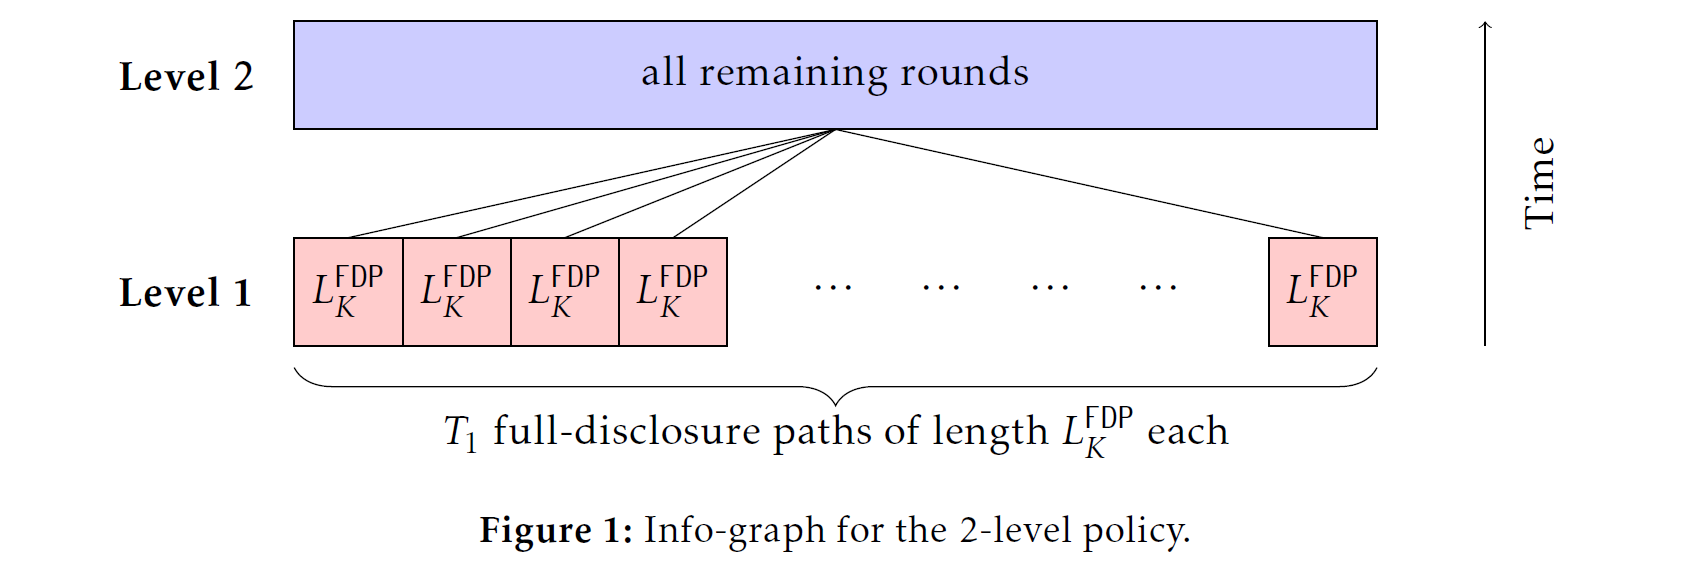
\includegraphics[width=0.99\linewidth]{2l.png} 
\end{center}
\textbf{Theorem:}
\[
Reg(T) \leq O_K (T^{2/3} (\log(T))^{1/3})
\]
\end{block}

\end{column} % End of the first column

\begin{column}{.01\textwidth}\end{column} % Empty spacer column

\begin{column}{.44\textwidth} % The second column
\begin{block}{Three-level Policy}

\begin{center}
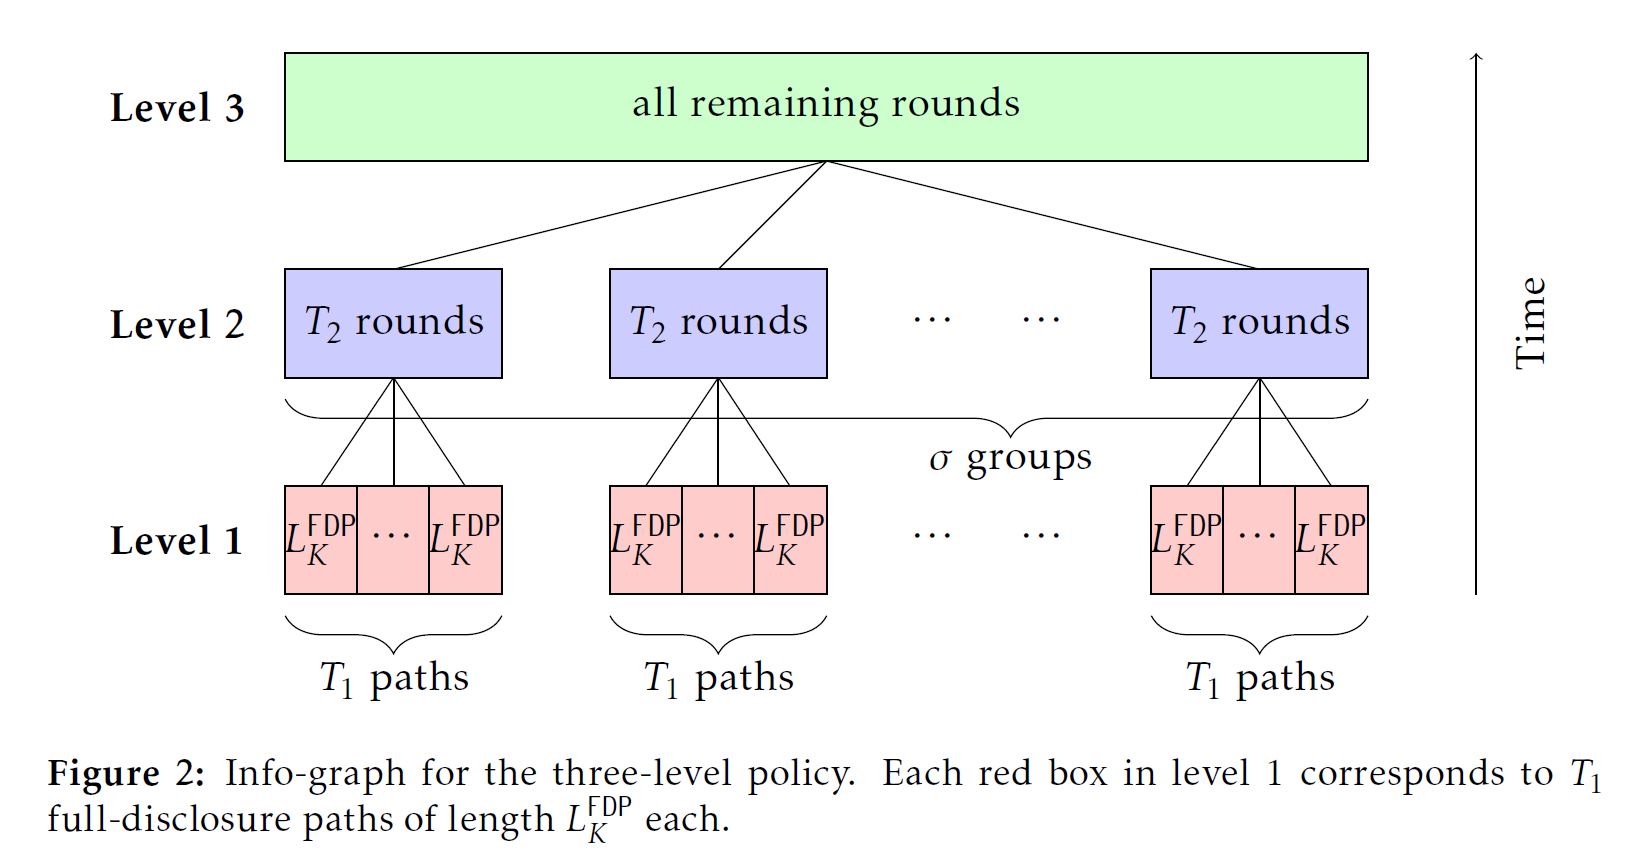
\includegraphics[width=0.99\linewidth]{3l.png} 
\end{center}
\textbf{Theorem:}
\[
Reg(T) \leq O_K (T^{4/7} \log(T))
\]
\textbf{Proof Sketch} (for 2 arms): Wlog $\mu_1 \geq \mu_2$,  $\Delta = \mu_1 - \mu_2$\\
$T_1 = T^{4/7} \log^{-1/7}(T)$, $T_2 = T^{6/7}\log^{-5/7}(T)$, $\sigma= \log(T)$\\
Case analysis based on $\Delta$:
\begin{itemize}
\item (Negligible gap) $\Delta < T^{-3/7}\log^{6/7}(T)$: \\picking any arm gives small regret\\
~
\item (Large gap) $\Delta > \sqrt{\log(T)/T_1} = T^{-2/7} \log^{4/7}(T)$:\\ concentration in the first level \\$\Rightarrow$ all agents in the second and the third levels pull arm 1\\~
\item (Small gap) $\Delta \in (T^{-3/7}\log^{6/7}(T), \sqrt{1/T_1})$:\\ anti-concentration in the first level \\$\Rightarrow$ both arms are pulled $\geq T_2$ times, concentration in the second level\\ $\Rightarrow$ all agents in the third level pull arm 1\\~
\item (Medium gap) $\Delta \in (\sqrt{1/T_1}, \sqrt{\log(T)/T_1})$:\\ concentration in the first level \\$\Rightarrow$ all agents in the third level pull arm 1
\end{itemize}
\end{block}

\begin{block}{$L$-level Policy}
\begin{center}
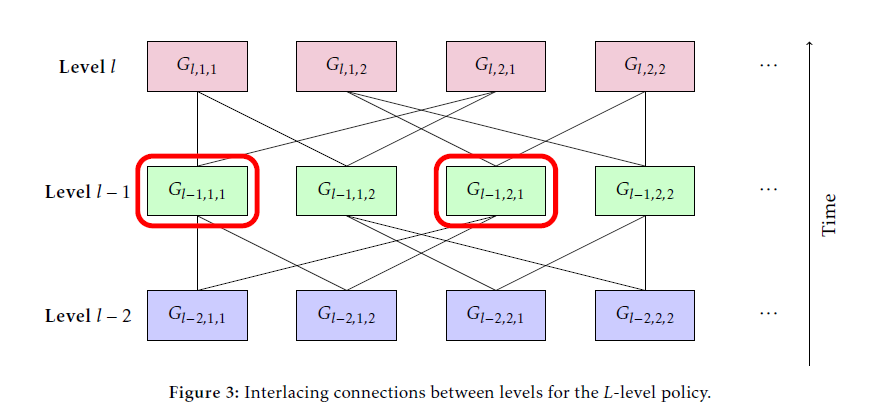
\includegraphics[width=0.99\linewidth]{ll.png} 
\end{center}
\textbf{Interlacing connection:} Agents in Group $G_{l,u,v}$ sees history of agents in group $G_{l-1,v,w}$ for all $u,v,w \in [\log(T)]$\\
~\\
\textbf{Theorem:}
$L$-level policy:
\[
Reg(T) \leq O_K (T^{2^{L-1} / (2^L-1)} \text{poly}\log(T))
\]
$O(\log(T)/\log\log(T))$-level policy:
\[
Reg(T) \leq O_K(T^{1/2} \text{poly} \log(T))
\]
\end{block}

\end{column} % End of the second column

\begin{column}{.01\textwidth}\end{column} % Empty spacer column

\end{columns} % End of all the columns in the poster

\end{frame} % End of the enclosing frame


\end{document}
